\documentclass[
  % -- opções da classe memoir --
  12pt,       % tamanho da fonte
  % openright,      % capítulos começam em pág ímpar (insere página vazia caso preciso)
  oneside,      % para impressão em verso e anverso, use twoside.
  a4paper,      % tamanho do papel. 
  % -- opções da classe abntex2 --
  %chapter=TITLE,   % títulos de capítulos convertidos em letras maiúsculas
  %section=TITLE,   % títulos de seções convertidos em letras maiúsculas
  %subsection=TITLE,  % títulos de subseções convertidos em letras maiúsculas
  %subsubsection=TITLE,% títulos de subsubseções convertidos em letras maiúsculas
  % -- opções do pacote babel --
  english,      % idioma adicional para hifenização
  %french,       % idioma adicional para hifenização
  %spanish,      % idioma adicional para hifenização
  brazil        % o último idioma é o principal do documento
  ]{abntex2}

% ---
% Pacotes básicos 
% ---
\usepackage{lmodern}      % Usa a fonte Latin Modern      
\usepackage[T1]{fontenc}    % Selecao de codigos de fonte.
\usepackage[utf8]{inputenc}   % Codificacao do documento (conversão automática dos acentos)
\usepackage{lastpage}     % Usado pela Ficha catalográfica
\usepackage{indentfirst}    % Indenta o primeiro parágrafo de cada seção.
\usepackage{color}        % Controle das cores
\usepackage{graphicx}     % Inclusão de gráficos
\usepackage{microtype}      % para melhorias de justificação
\usepackage{amsmath}      % para fórmulas matemáticas
\usepackage{amssymb}      % para símbolos matemáticos

% ---
% Pacotes de citações
% ---
\usepackage[brazilian,hyperpageref]{backref}   % Paginas com as citações na bibl
\usepackage[alf]{abntex2cite} % Citações padrão ABNT

% --- 
% CONFIGURAÇÕES DE PACOTES
% --- 

% ---
% Configurações do pacote backref
% Usado sem a opção hyperpageref de backref
\renewcommand{\backrefpagesname}{Citado na(s) página(s):~}
% Texto padrão antes do número das páginas
\renewcommand{\backref}{}
% Define os textos da citação
\renewcommand*{\backrefalt}[4]{
  \ifcase #1 %
    Nenhuma citação no texto.%
  \or
    Citado na página #2.%
  \else
    Citado #1 vezes nas páginas #2.%
  \fi}%
% ---

% ---
% Informações de dados para CAPA e FOLHA DE ROSTO
% ---
\titulo{Heurísticas para Predição de Configurações de\\ Custo Mínimo para Execução de Aplicações em Ambientes de Nuvem de Infraestrutura}
\autor{Marcelo Canário Gonçalves}
\orientador{Prof. Dr. Américo Tadeu Falcone Sampaio}
\coorientador{Prof. Dr. Nabor das Chagas Mendonça}
\instituicao{%
  Universidade de Fortaleza
  \par
  Programa de Pós-Graduação em Informática Aplicada (PPGIA)}
\local{FORTALEZA}
\data{2014}
\tipotrabalho{Dissertação (Mestrado)}

% O preambulo deve conter o tipo do trabalho, o objetivo, 
% o nome da instituição e a área de concentração 
\preambulo{Dissertação apresentada ao Programa de Pós-Graduação em Informática
Aplicada (PPGIA) da Universidade de Fortaleza como parte dos requisitos
necessários para a obtenção do grau de Mestre em Informática Aplicada.}
% ---

% ---
% Configurações de aparência do PDF final

% alterando o aspecto da cor azul
\definecolor{blue}{RGB}{41,5,195}

% informações do PDF
\makeatletter
\hypersetup{
      %pagebackref=true,
    pdftitle={\@title}, 
    pdfauthor={\@author},
      pdfsubject={\imprimirpreambulo},
      pdfcreator={LaTeX with abnTeX2},
    pdfkeywords={abnt}{latex}{abntex}{abntex2}{trabalho acadêmico}, 
    %colorlinks=false,          % false: boxed links; true: colored links
      linkcolor=blue,           % color of internal links
      %citecolor=blue,           % color of links to bibliography
      filecolor=magenta,          % color of file links
    urlcolor=blue,
    bookmarksdepth=4
}
\makeatother
% --- 

% --- 
% Espaçamentos entre linhas e parágrafos 
% --- 

% O tamanho do parágrafo é dado por:
\setlength{\parindent}{1.3cm}

% Controle do espaçamento entre um parágrafo e outro:
\setlength{\parskip}{0.2cm}  % tente também \onelineskip

%Altera a capa
% Impressão da Capa
\renewcommand{\imprimircapa}{%
\begin{capa}%
\center

% Logomarca da Universidade

\includegraphics[scale=2]{./img/logo.png}\\
\textbf{FUNDAÇÃO EDSON QUEIROZ}\\
\textbf{UNIVERSIDADE DE FORTALEZA -- UNIFOR}

\vfill
\ABNTEXchapterfont\bfseries\LARGE\imprimirtitulo
\vfill

\ABNTEXchapterfont\large\imprimirautor
\vspace*{1cm}
\vfill\vfill\vfill
\large\imprimirlocal

\large\imprimirdata

\vspace*{1cm}
\end{capa}
}
% ---
% Altera a folha de rosto
\renewcommand{\folhaderostocontent}{
  \begin{center}

    {\ABNTEXchapterfont\large\imprimirautor}

    \vspace*{\fill}\vspace*{\fill}
    \begin{center}
      \ABNTEXchapterfont\bfseries\Large\imprimirtitulo
    \end{center}
    \vspace*{\fill}

    \hspace{.45\textwidth}
    \begin{minipage}{.5\textwidth}
      \SingleSpacing
      \imprimirpreambulo
    \end{minipage}%
    \vspace*{\fill}

    {\large\imprimirorientadorRotulo~\imprimirorientador\par}
    {\large\imprimircoorientadorRotulo~\imprimircoorientador}%
    \vspace*{\fill}

    {\imprimirinstituicao\vspace*{\fill}}

    {\large\imprimirlocal}
    \par
    {\large\imprimirdata}
    \vspace*{1cm}

  \end{center}
}


% ---
% compila o indice
% ---
\makeindex
% ---

% ----
% Início do documento
% ----
\begin{document}

% Retira espaço extra obsoleto entre as frases.
\frenchspacing 

% ----------------------------------------------------------
% ELEMENTOS PRÉ-TEXTUAIS
% ----------------------------------------------------------
% \pretextual

% ---
% Capa
% ---
\imprimircapa
% ---

% ---
% Folha de rosto
% (o * indica que haverá a ficha bibliográfica)
% ---
\imprimirfolhaderosto*

% ---
% Inserir a ficha bibliografica
% ---
% Isto é um exemplo de Ficha Catalográfica, ou ``Dados internacionais de
% catalogação-na-publicação''. Você pode utilizar este modelo como referência. 
% Porém, provavelmente a biblioteca da sua universidade lhe fornecerá um PDF
% com a ficha catalográfica definitiva após a defesa do trabalho. Quando estiver
% com o documento, salve-o como PDF no diretório do seu projeto e substitua todo
% o conteúdo de implementação deste arquivo pelo comando abaixo:
%
% \begin{fichacatalografica}
%     \includepdf{fig_ficha_catalografica.pdf}
% \end{fichacatalografica}
\begin{fichacatalografica}
  \vspace*{\fill}         % Posição vertical
  \hrule              % Linha horizontal
  \begin{center}          % Minipage Centralizado
  \begin{minipage}[c]{12.5cm}   % Largura
  
  \imprimirautor
  
  \hspace{0.5cm} \imprimirtitulo  / \imprimirautor. --
  \imprimirlocal, \imprimirdata-
  
  \hspace{0.5cm} \pageref{LastPage} p. : il. (algumas color.) ; 30 cm.\\
  
  \hspace{0.5cm} \imprimirorientadorRotulo~\imprimirorientador\\
  
  \hspace{0.5cm}
  \parbox[t]{\textwidth}{\imprimirtipotrabalho~--~\imprimirinstituicao,
  \imprimirdata.}\\
  
  \hspace{0.5cm}
    1. Cloud computing.
    2. Heurísticas.
    I. Orientador.
    II. Universidade de Fortaleza.
    III. PPGIA.
    IV. Título\\      
  
  \hspace{8.75cm} CDU 02:141:005.7\\
  
  \end{minipage}
  \end{center}
  \hrule
\end{fichacatalografica}
% ---


% ---
% Inserir folha de aprovação
% ---
% Isto é um exemplo de Folha de aprovação, elemento obrigatório da NBR
% 14724/2011 (seção 4.2.1.3). Você pode utilizar este modelo até a aprovação
% do trabalho. Após isso, substitua todo o conteúdo deste arquivo por uma
% imagem da página assinada pela banca com o comando abaixo:
%
% \includepdf{folhadeaprovacao_final.pdf}
%
\begin{folhadeaprovacao}

  \begin{center}
    {\ABNTEXchapterfont\large\imprimirautor}

    \vspace*{\fill}\vspace*{\fill}
    \begin{center}
      \ABNTEXchapterfont\bfseries\Large\imprimirtitulo
    \end{center}
    \vspace*{\fill}
    
%    \hspace{.45\textwidth}
%    \begin{minipage}{.5\textwidth}
%        \imprimirpreambulo
%    \end{minipage}%
%    \vspace*{\fill}
           
   Data de aprovação: 15 de dezembro de 2014.

   \assinatura{\textbf{\mbox{\imprimirorientador}} \\ (Orientador -- UNIFOR)} 
   \assinatura{\textbf{\mbox{\imprimircoorientador}} \\(Coorientador -- UNIFOR)}%
   
   \assinatura{\textbf{\mbox{Prof. Dr. Danielo Gonçalves Gomes}} \\ (Membro -- UFC)}
    \assinatura{\textbf{\mbox{Prof. Dr. Pedro Porfírio Muniz Farias}} \\ (Membro -- UNIFOR)}
   %\assinatura{\textbf{Professor} \\ Convidado 3}
   %\assinatura{\textbf{Professor} \\ Convidado 4}
      
      
   \begin{center}
    \vspace*{\fill}
    %\vspace*{0.5cm}
    {\large\imprimirlocal}
    \par
    {\large\imprimirdata}
    \vspace*{1cm}
   \end{center}
   
   \end{center}
  
\end{folhadeaprovacao}
% ---


% ---
% Dedicatória
% ---
\begin{dedicatoria}
   \vspace*{\fill}
   \centering
   \noindent
   \textit{ À minha esposa, meu Anjo e minha luz, Isabela,\\
   e à minha filha e razão de viver, Melisa.} \vspace*{\fill}
\end{dedicatoria}
% ---


% ---
% Agradecimentos
% ---
\begin{agradecimentos}
Deus, Isabela e Mel, Mãe(orações de longe)\\ 
Chagas, Bento, -- liberação e suporte\\
Jaime Gama, Paulo Benicio, José Maria -- cartas de recomendacao\\
Matheus, -- colaboração\\
Américo e Nabor,\\
Julio e Ronaldo, -- momentos de dificuldade e horas de laboratorio\\
\end{agradecimentos}
% ---


% ---
% Epígrafe
% ---
\begin{epigrafe}
    \vspace*{\fill}
  \begin{flushright}
    \emph{``Porque um dia é preciso parar de sonhar, \\
    tirar os planos da gaveta e, \\
    de algum modo, começar.'' \\
    Amyr Klink}
  \end{flushright}
  \begin{flushright}
    \emph{``O que importa é o conhecimento'' \\
    Sabedoria baiana}
  \end{flushright}
\end{epigrafe}


% ---


% ---
% RESUMOS
% ---
% resumo em português
\setlength{\absparsep}{18pt} % ajusta o espaçamento dos parágrafos do resumo
\begin{resumo}
Um dos principais desafios enfrentados pelos usuários de nuvens que oferecem 
infraestrutura-como-serviço (IaaS) é planejar adequadamente a capacidade dos 
recursos da nuvem necessários às suas aplicações. Este trabalho propõe uma nova 
abordagem para apoiar o planejamento da capacidade de aplicações em nuvens IaaS. 
A nova abordagem tem como premissa a definição de uma relação de capacidade 
entre as diferentes configurações de recursos oferecidas por um provedor de nuvem, 
com a qual é possível prever (ou ``inferir''), com alto grau de precisão, o 
desempenho esperado de uma aplicação para determinadas configurações de recursos. 
A predição é realizada com base no desempenho observado para outras configurações 
de recursos do mesmo provedor. Dessa forma, a abordagem consegue reduzir, de 
forma significativa, o número total de configurações que precisam ser de fato 
testadas na nuvem (resultados preliminares, obtidos em um ambiente real de nuvem, 
mostram uma redução de mais de 80\% no número total de configurações avaliadas), 
implicando em menores custo e tempo para o processo de planejamento.

 \textbf{Palavras-chaves}: Computação em Nuvem. Planejamento de Capacidade. Inferência de Desempenho.
\end{resumo}

% resumo em inglês
\begin{resumo}[Abstract]
 \begin{otherlanguage*}{english}
One of the main challenges faced by users of Infrastructure-as-a-Service (IaaS) 
clouds is to correctly plan the resource capacity required for their applications'
needs. This work proposes a new approach to support application capacity planning 
in IaaS clouds. This new approach is based on the definition of a capacity relation 
between different resource configurations offered by a cloud provider which allows 
the prediction (or ``inference''), with a high level of accuracy, of the expected performance 
of an application for certain resource configurations. The prediction is made based
upon the observed performance for other resource configurations within the same 
provider. The approach significantly reduces the total number of configurations 
effectively tested in the cloud (preliminary results show reductions of over 80\% 
on the number of total tested configurations) resulting in lower time and financial costs  
for the capacity planning process.

   \vspace{\onelineskip}
 
   \noindent 
   \textbf{Key-words}: Cloud Computing. Capacity Planning. Performance Inference.
 \end{otherlanguage*}
\end{resumo}


% ---
% listas de ilustrações, tabelas, abreviaturas, siglas e símbolos
% ---
% ---
% inserir lista de ilustrações
% ---
\pdfbookmark[0]{\listfigurename}{lof}
\listoffigures*
\cleardoublepage
% ---

% ---
% inserir lista de tabelas
% ---
\pdfbookmark[0]{\listtablename}{lot}
\listoftables*
\cleardoublepage
% ---

% ---
% inserir lista de abreviaturas e siglas
% ---
\begin{siglas}
  \item[ABNT] Associação Brasileira de Normas Técnicas
  \item[abnTeX] ABsurdas Normas para TeX
\end{siglas}
% ---

% ---
% inserir lista de símbolos
% ---
\begin{simbolos}
  \item[$ \Gamma $] Letra grega Gama
  \item[$ \Lambda $] Lambda
  \item[$ \zeta $] Letra grega minúscula zeta
  \item[$ \in $] Pertence
\end{simbolos}
% ---


% ---
% inserir o sumario
% ---
\pdfbookmark[0]{\contentsname}{toc}
\tableofcontents*
\cleardoublepage
% ---


% ----------------------------------------------------------
% ELEMENTOS TEXTUAIS
% ----------------------------------------------------------
\textual

% ----------------------------------------------------------
% Introdução
% ----------------------------------------------------------
\chapter[Introdução]{Introdução}
% ----------------------------------------------------------
O processo de decisão pela migração de aplicações para o ambiente de nuvens computacionais 
envolve uma série de análises que buscam, entre outras coisas, identificar que vantagens a 
mudança trará de fato. Ao comparar os serviços de provedores de computação em nuvem com a 
administração de um centro de dados próprio, a melhoria dos indicadores de desempenho e de 
custo, como redução de tempo de resposta, redução/otimização de custo de operação e melhores 
ferramentas com mais facilidades de gerenciamento, está entre os principais benefícios buscados 
a partir da adoção do ambiente de infraestrutura como serviço (IaaS – Infrastructure as a Service)
\cite{li2011cloudprophet, rodero2010infrastructure}.

Em geral, provedores de IaaS cobram um valor em função do tempo de ocupação de uma máquina 
virtual, normalmente medido em horas, e esse valor unitário varia conforme o tamanho da máquina 
virtual (capacidade de processamento, memória e espaço de armazenamento). Dessa forma, a apuração 
do custo de operação da aplicação em um determinado período de tempo leva em conta a quantidade 
de máquinas virtuais utilizadas bem como seu perfil, ou seja, o tamanho e quantidade de recursos 
usados em cada uma.
 
Para prever o custo de operação de uma aplicação na nuvem, é preciso estimar ou medir como a 
aplicação responderá à demanda submetida em termos de indicadores de desempenho. A aplicação deve 
manter ou superar na nuvem o nível de desempenho apresentado quando executada em centro de dados 
próprio e com indicadores de custo menores, a fim de que se justifique o investimento feito na 
migração de ambiente. Para se chegar a essa conclusão, faz-se necessário conhecer o comportamento 
da aplicação na nova implantação para que se identifiquem quais perfis de máquinas virtuais 
oferecidos pelo provedor são capazes de executar a aplicação com níveis satisfatórios de desempenho. 
Somem-se a isso as variações da demanda exercida sobre a aplicação e as diversas possibilidades de 
variação de arquitetura de implantação por meio de procedimentos de escalabilidade.
 
Ao se tomarem procedimentos de escalabilidade vertical (variando-se a quantidade de recursos de 
cada máquina) e/ou de escalabilidade horizontal (variando-se a quantidade de máquinas em uma ou 
mais camadas da aplicação, como dados, apresentação e negócio) chega-se a níveis de desempenho e de custo muito 
diversos. A variação da demanda exige que a aplicação também varie em tamanho da implantação, 
vertical ou horizontalmente, conforme a carga aplicada. Quanto mais acentuadas e mais frequentes 
as variações na demanda, mais variações de custo e desempenho serão observadas.

Assim, o custo apresenta-se entre os mais difíceis de prever, uma vez que depende necessariamente 
do tamanho da demanda exercida sobre a aplicação além do desempenho oferecido e preços cobrados 
pelo provedor de nuvem de infraestrutura contratado \cite{cunha2012ambiente}. Estrategicamente, 
torna-se interessante identificar, entre as possíveis composições de máquinas virtuais ofertadas 
em um ou vários provedores, quais são as configurações de menor custo capazes de executar a 
aplicação mantendo-se os níveis satisfatórios para os indicadores de desempenho.

Para saber se uma determinada configuração de recursos do provedor é capaz de atender a uma 
demanda específica, é preciso antes enumerar os indicadores de desempenho que mais interessam 
à aplicação e a partir daí estabelecer os valores aceitáveis para esses indicadores. Uma vez 
estabelecidos os valores aceitáveis, pode-se implantar a aplicação sob essa configuração de 
recursos e então aplicar diferentes níveis de carga de trabalho sobre a aplicação. Ao comparar 
a resposta da aplicação com os valores dados como aceitáveis para os indicadores, é possível 
determinar se aquela configuração de recursos escolhida é capaz de executar a aplicação a 
contento e ainda calcular o custo mensal dessa implantação.

Porém, partindo-se do pressuposto de que o desempenho da aplicação foi satisfatório, o que se 
tem até agora é o custo de uma única configuração capaz de executar a aplicação estudada sob 
um único nível de carga de trabalho. No entanto, cargas de trabalho costumam variar em função do tempo 
em implantações reais, fazendo-se necessário, portanto, que esse efeito seja contemplado nos 
testes por meio da medição do desempenho da aplicação submetida a diferentes níveis de carga 
de trabalho.

Analogamente, as diversas configurações de máquinas e recursos, ainda que no mesmo provedor, 
podem responder de maneira muito diferente sob o mesmo nível de carga de trabalho a depender 
do momento em que sejam ativados \cite{cunha2011investigating, iosup2011performance, 
jayasinghe2011variations}. Independente do motivo que leve a esse comportamento de certa 
forma imprevisível, é preciso levar em conta nos ensaios de avaliação de desempenho essa 
variabilidade e isso pode ser alcançado através da repetição dos cenários de teste em horários 
e dias diferentes.

Um grande problema começa a se desenhar ao seguir essa abordagem: a fase de ensaios pode atingir 
patamares elevados de custo, a depender das necessidades de variação da demanda, da arquitetura 
de implantação e das configurações utilizadas em cada arquitetura implantada 
\cite{silva2013cloudbench}. Ainda que certos provedores IaaS ofereçam descontos ou pacotes de 
horas grátis para novos clientes, em geral esses incentivos são suficientes para custear apenas 
um mês de utilização de uma única máquina virtual muito pequena, provavelmente incapaz de suportar 
a carga de uma aplicação real em produção. Assim, executar uma aplicação real, tipicamente 
implantada em arquitetura de várias camadas, em máquinas virtuais de tamanho considerável e por 
longos períodos de tempo apenas para estudar o seu comportamento, pode se traduzir em um custo 
alto que inviabilize o próprio projeto de migração dessa aplicação para a nuvem. Para evitar 
que sejam feitos testes com todas as combinações de provedores, configurações, horários, cargas 
de trabalho e métricas avaliadas, é possível lançar mão de técnicas de predição.

Através da predição, é possível estimar com razoável aproximação o desempenho que a aplicação 
apresentará ao ser executada em vários perfis de configuração diferentes, permitindo a 
determinação de qual configuração de menor custo capaz de executar a aplicação e sem a 
necessidade da realização completa dos testes. Como consequência, o custo dessa fase de 
ensaios pode ser reduzido sensivelmente.

Este trabalho propõe heurísticas de predição de custo mínimo para execução de aplicações 
em ambientes de nuvem de infraestrutura, bem como um arcabouço de programação que apoia a 
implementação dessas heurísticas. Além disso, o trabalho estuda os resultados apresentados 
pela aplicação das heurísticas propostas quanto ao custo total de execução da fase de ensaios 
para escolha da melhor configuração capaz de executar uma aplicação e quanto à acuidade dos 
resultados da predição em si.

% ----------------------------------------------------------

% ----------------------------------------------------------
% Trabalhos Relacionados
% ----------------------------------------------------------
\chapter[Trabalhos Relacionados]{Trabalhos Relacionados}
% ----------------------------------------------------------
Apresentamos  neste capítulo alguns trabalhos cujos objetivos estejam alinhados 
com a ideia da avaliação de desempenho de aplicações executadas em ambientes de
computação em nuvem. Esses trabalhos estão agrupados de acordo com a abordagem utilizada para a realização da avaliação de desempenho. São duas abordagens, a primeira é a abordagem preditiva, nesta, os trabalhos não executam diretamente a aplicação alvo no ambiente onde se deseja implantá-la. Já a segunda abordagem é a empírica, nesta as aplicações alvo são implantadas na nuvem e então submetidas a testes de carga. 

Para apoiar a análise crítica de cada trabalho e suas abordagens, definimos um conjunto de critérios a partir dos quais poderemos tanto descrever, quanto comparar as soluções existentes de apoio a avaliação de desempenho do ponto de vista do usuário. Seguem os critérios:

\begin{enumerate}
  \item Completude da solução
  \begin{enumerate}
    \item Definição da aplicação --- flexibilidade da solução para
    definir a aplicação a ser avaliada;
    \item Definição da demanda --- flexibilidade da solução para
    definir os níveis de carga de trabalho sobre os quais a aplicação será
    submetida;
	\item Definição dos recursos da nuvem --- flexibilidade da solução para
	definir as configurações de recursos do provedor sobre as quais a aplicação
	será executada;
	\item Definição do acordo de nível de serviço (SLA) --- flexibilidade da
	solução para definir o SLA desejado.
  \end{enumerate}
  \item Efetividade da solução  
  \begin{enumerate}
    \item Eficiência --- tempo e custo necessários para a solução resolver o
    problema;
    \item Acurácia --- confiabilidade das respostas oferecidas pela solução;
	\item Complexidade --- grau de complexidade/esforço exigido do usuário da
	solução.
  \end{enumerate}
\end{enumerate}

Cada abordagem será apresentada em uma subseção, bem como os diversos trabalhos da área que serão resumidos separadamente. Ao final da subseção, será apresentada uma análise crítica que será baseada nos critérios descritos acima.

\section{Ferramentas com Abordagem Preditiva}
\subsection{Cloud Harmony}
O projeto {\em CloudHarmony}, cujo
objetivo é ``tornar-se a principal fonte independente, imparcial e útil de
métricas de desempenho de provedores de nuvem''~\cite{cloudharmony}, agrega
dados de testes de desempenho realizados desde 2009 em mais de 60 provedores de
nuvem. Além do histórico das avaliações, o {\em CloudHarmony} disponibiliza uma ferramenta para executar novas avaliações de desempenho a qualquer momento, denominada
\textit{Cloud Speed Test},\footnote{\url{http://cloudharmony.com/speedtest}}, a qual permite realizar quatro tipos de teste:

\begin{description}
  \item[\em Download a few large files] --- objetiva determinar o melhor provedor
  para descarregar arquivos grandes, sendo útil para aplicações como {\em video
  streaming};
  \item[\em Download many small files] --- objetiva determinar o melhor provedor
  para descarregar arquivos pequenos, podendo ser útil para hospedar uma página
  web, por exemplo;
  \item[\em Upload] --- útil para avaliar serviços que serão utilizados para
  envio de arquivos;
  \item[\em Test network latency] --- a latência afeta o tempo de resposta da
  aplicação e geralmente está relacionada com a região de onde o teste está
  partindo.
\end{description}

Os resultados disponibilizados pelo {\em CloudHarmony} têm como pontos fortes a
grande quantidade de dados de testes de desempenho disponíveis, além da possibilidade do cliente da
nuvem poder executar novos testes a qualquer tempo. Por outro lado, os testes estão limitados àqueles implementados pela ferramenta de teste, não podendo ser facilmente modificados para contemplar novas métricas ou cenários de avaliação.

\subsection{{\em CloudXplor}}

{\em CloudXplor}~\cite{malkowski2010cloudxplor} é uma ferramenta para
planejamento de configuração de recursos da nuvem baseada em dados empíricos. A ferramenta
foi desenvolvida tomando como base um modelo de planejamento de configuração de
recursos de Tecnologia da Informação (TI), com foco explícito em aspectos econômicos.
Por essa razão, a ferramenta se utiliza de acordos de nível de serviço baseados na relação do custo
da infraestrutura de TI com o valor dos recursos do provedor do serviço. Esse
valor será maior quando o tempo de resposta da aplicação for plenamente atendido
pelo provedor do serviço, e vai diminuindo à medida em que esse tempo de resposta
não é alcançado.

Os dados empíricos precisam ser coletados, previamente, através da execução de diversos experimentos de avaliação de desempenho. Esses dados
são compostos por métricas de sistema (uso de CPU, memória utilizada, tráfego na rede e E/S de disco) e métricas de mais alto nível (tempo de resposta e \textit{throughput}). Após a coleta, os dados dos experimentos são submetidos e analisados pela ferramenta, utilizando um de seus quatro módulos: análise de tempo de
resposta, análise de \textit{throughput}, análise do valor agregado e do custo,
e análise do lucro. Cada um desses módulos filtra os dados, fazendo uso apenas
das informações necessárias para a execução da sua análise. Após a análise dos
 dados, a ferramenta pode ser utilizada para produzir gráficos que ilustram o comportamento da aplicação ao se variar
parâmetros como carga de trabalho e configuração dos componentes da aplicação.


A ferramenta proposta no trabalho faz uso de dados previamente coletados
e só então realiza a análise do desempenho de aplicações na nuvem
em diversos recursos. Por isso deixa a cargo do cliente da nuvem todas as
atividades para a avaliação de desempenho, pois depende dos dados empíricos que
são coletados após a avaliação. O CloudXplor é capaz de plotar um gráfico com o
comportamento da aplicação à medida em que é exposta a variação na demanda, do
custo e do valor, mas só o faz por que o cliente da nuvem executou cada uma das
avaliações manualmente. Da mesma forma a variação na demanda vai depender do
conjunto de avaliações executadas pelo cliente da nuvem, a ferramenta apenas
plota gráficos do que foi executado pelo cliente. Com relação a definição de
cenários de avaliação e a definição de parâmetros de desempenho, a ferramenta
não dá nenhum suporte, uma vez que os cenários dependem das avaliações
realizadas e que os módulos de análise de custo, valor, tempo de resposta e {\em
throughput} possuem uma lista dos parâmetros de desempenho possíveis de
avaliação.


\subsection{CloudCmp}
\citeonline{li2011} apresentam uma ferramenta para apoiar a avaliação e a comparação do
desempenho e do custo dos recursos e serviços de diversos provedores de nuvem
pública, de modo a auxiliar o cliente da nuvem a escolher o provedor mais adequado para a sua
aplicação. Essa ferramenta, denominada {\em CloudCmp}, analisa
os serviços de elasticidade, persistência de dados e rede oferecidos pelos provedores
de interesse, com base em resultados previamente coletados a partir da execução de diversos
{\em benchmarks}: uma versão modificada do {\em SPECjvm2008}~\cite{SPECjvm2008}
para avaliar a característica de elasticidade do provedor; um cliente Java para avaliar os serviços de
armazenamento e persistência de dados; e as ferramentas {\em iperf}\footnote{http://iperf.sourceforge.net. }
e {\em ping} para avaliar os serviços de rede. Após a fase inicial da coleta dos dados, a ferramenta pode ser utilizada para gerar gráficos que auxiliem o
cliente da nuvem a comparar o desempenho dos recursos de cada um
dos provedores nos quais as avaliações foram realizadas, que assim poderá escolher o provedor e os recursos mais apropriados para as necessidades e demandas específicas de suas aplicações. 

%Os gráficos gerados nos
%experimentos apresentados neste trabalho foram comparados com os gerados após o
%estudo do comportamento de três aplicações simples implantadas na nuvem. Essas
%comparações mostraram que as previsões do CloudCmp refletiram o comportamento
%das aplicações testadas.

Segundo \citeonline{li2011}, até a época do trabalho não houve
nenhum provedor de nuvem que se destacasse com relação aos demais. Outra constatação foi de que os resultados
obtidos a partir da execução dos {\em benchmarks} em cada provedor apenas refletiam o momento em que foram coletados, uma vez que a estrutura utilizada pelos provedores para hospedar seus serviços sofre frequentes modificações e a demanda por seus recursos computacionais é bastante variável.

Como essa solução compara serviços e recursos da nuvem através da análise de dados
previamente coletados a partir da execução de diferentes {\em benchmarks}, a
escolha dos provedores e recursos mais apropriados para uma determinada aplicação só será eficaz se a aplicação utilizar os recursos da nuvem de forma semelhante à dos {\em benchmarks} avaliados. Além disso, a
ferramenta não oferece suporte à execução de novos cenários de avaliação na nuvem, estando limitada àqueles previamente definidos para os respectivos {\em bechmarks}.

\subsection{CloudAdvisor}
O trabalho apresentado em~\cite{jung2013cloudadvisor} ``introduz uma nova plataforma de recomendação de nuvem, chamada {\em CloudAdvisor}''. Essa plataforma destina-se a auxiliar o seu usuário na tarefa de capturar as implicações monetárias e financeiras das configurções de implantação das suas aplicações. Para recomendar a configuração, a platforma recebe como entrada parâmetros de configuração de alto nível como, orçamento, expectativa de performance e economia de energia, os quais estão limitados a uma escala discreta que vai de 0 até 10, onde 0 significa baixa influência e 10 significa alta influência. Uma vez informados os parâmetros de configuração, o {\em CloudAdvisor} irá caracterizar a performance da aplicação alvo em termos de uso dos recursos computacionais e em seguida executará o {\em benchmark} {\em CloudMeter},~\cite{jung2013cloudadvisor}, nas nuvens candidatas, a fim de caracterizar a performance dos recursos dessas nuvens.

Para ilustrar o uso do {\em CloudAdvisor}, os autores implantaram a solução em servidores locais e em três provedores de nuvem pública, foram eles: Windows Azure, Rackspace, and Amazon EC2. Como resultado, foi observado que a taxa de erro da configuração para uma determinada carga foi de 10~\%. No entanto, quando o usuário do ambiente escolhe parâmetros de configuração extremos (por exemplo, configurar o máximo de orçamento, de economia de energia e de nível de performance), essa taxa de erro elevou para 18~\%.

Os autores concluem que o usuário da solução pode explorar diversas opções de configuração da sua aplicação na nuvem utilizando uma interface amigável e sem a necessidade de informar detalhes específicos de configuração. Além disso, mostraram que é possível utilizar uma técnica de caracterização de performance, para uma dada carga, baseada na execução de {\em benchmarks} em nuvens candidatas.

\subsection{CDOSim}
Uma solução para o desafio da escolha da configuração de implantação de uma aplicação na nuvem foi apresentada em~\cite{fittkau2012cdosim} com o nome de \textit{CDOSim}. Essa ferramenta auxilia o usuário no processo de escolha do que os autores chamaram de opção de implantação na nuvem, do inglês \textit{Cloud Deployment Option} (CDO). Uma vez que a análise manual das ``potenciais CDOs é intratável, custosa e consome tempo, devido à heterogeneidade dos ambientes de nuvem'',~\cite{fittkau2012cdosim}. Para a escolha das CDOs, são realizadas simulações que se baseiam no custo e nas propriedades de performance de cada CDO. Como requisito para a utilização de uma CDO nas simulações, é preciso caracterizar as suas propriedades de performance em termos de \textit{mega integer plus instructions per second} (MIPIPS)~\cite{fittkau2012cdosim}, essa caracterização é realizada através da execução de um \textit{benchmark} cujo código é gerado para cada linguagem de programação utilizada pela aplicação alvo. Esta, por sua vez, deve passar por um processo de engenharia reversa para modelos KDM, que é descrito em~\cite{perez2011knowledge}, para que o simulator consiga escolher a opção de configuração mais adequada.

Para validar o \textit{benchmark} MIPIPS, os resultados da simulação em comparação com dados reais e a predição da performance de um provedor de nuvem com base nos dados de outro provedor de nuvem, os autores conduziram uma série de experimentos em dois ambientes de nuvem, uma pública a Amazon EC2 e outra privada. Na nuvem pública foi evidenciado que os valores de MIPIPS dependem da região onde o \textit{benchmark} foi realizado e da carga sobre a máquina física que hospeda a vitual. Já na comparação dos resultados da simulação com os dados reais, os autores mostraram que a taxa de error da utilização de CPU simulada com a utilização de CPU medida chegou a 30,86~\%, contudo, como a taxa de erro médio global foi abaixo de 22,75~\%, abaixo do threshold estabelecido pelos autores que era de 30~\%. Já a predição da performance de uma instância da Amazon EC2 a partir da performance de uma instância da nuvem privada gerou um 15,76~\% como taxa de erro global.

Finalmente, os autores concluem que a simulação pode auxiliar no processo de escolha da opção de implantação com maior performance e menor custo e que os resultados da simulação são razoavelmente próximos dos experimentos realizados dos valores reais.

\subsection{CloudProphet}
Em \cite{li2011cloudprophet} os autores apresentam o \textit{CloudProphet}, um sistema de
predição de desempenho de aplicações em ambiente de nuvem computacional baseado 
na metodologia de ``rastrear e reproduzir'' (\textit{trace and replay}).

O \textit{CloudProphet} não testa a aplicação do cliente de fato no ambiente de nuvem. De
modo contrário, ele injeta na implantação original da aplicação um módulo que 
registra um rastreamento detalhado dos eventos de utilização de recursos de CPU,
armazenamento e rede em cada componente da aplicação durante um período de 
execução habitual em seu ambiente de produção.

Em um passo seguinte, outro módulo faz uma extração das relações de dependência 
entre os eventos coletados, ordenando as transações executadas nos diversos 
componentes.

O terceiro passo é a reprodução dos eventos coletados durante a fase de 
rastreamento. Essa reprodução consiste fazer com que o ambiente de nuvem 
computacional que se deseja avaliar execute as transações representadas nos dados
do rastreamento a partir de requisições que partem de clientes simulados.
   
O objetivo do \textit{CloudBench}, segundo os autores é eliminar o custo e o trabalho 
envolvidos na migração da aplicação real para a nuvem para a execução de testes 
antes que seja de fato tomada a decisão em favor dessa migração.

Os autores argumentam que a simples implantação da aplicação no ambiente de um
serviço de nuvem computacional já incorre em custos, que podem ser altos a 
depender do tamanho ou da arquitetura da aplicação. Além disso, a tarefa de
migração pode ser bastante trabalhosa conforme o número e a diversidade dos 
componentes da aplicação, que podem acarretar dificuldades de configuração e
compatibilidade no novo ambiente.

\section{Ferramentas com Abordagem Empírica}
As ferramentas que serão apresentadas nesta seção têm em comum o fato de utilizarem como aplicação alvo a prória aplicação que se deseja implantar na nuvem. Portanto, é preciso inicialmente realizar uma implantação na nuvem para que seja dado início ao processo de análise de desempenho. Por isso, cada ferramenta oferece um mecanismo para que o seu usuário possa definir como a aplicação deve ser implantada e configurada. Além da definição da aplicação e dos recursos da nuvem que serão utilizados, essas ferramentas também permitem que sejam definidas a demanda que será imposta a cada aplicação e o acordo de nível de serviço. Dessa forma, é possível definir, por exemplo, o número de usuários simultâneos e o tempo de resposta esperado para uma transação.

Uma vez que que as ferramentas que realizam a abordagem empírica possibilitam ao usuário muita liberdade na definição da aplicação, demanda, recurso da nuvem e SLA, essas soluções têm o mais alto grau de completude. Além disso, como faz-se uso da própria aplicação alvo para a avaliação de desempenho, a acurácia dos resultados apresentados pelas ferramentas é a mais elevada. A seguir, apresentaremos quatro trabalhos que se destacam na avaliação de desempenho de aplicações na nuvem usando a abordagem empírica, são eles:~\cite{jayasinghe2012},~\cite{silva2013cloudbench},~\cite{cunhacloud},~\cite{scheuner2014cloud}.

\subsection{Expertus}
Devido à complexidade e às implicações da escolha da configuração para a implantação de uma aplicação na nuvem, em~\cite{jayasinghe2012} os autores apresentam o \textit{Expertus}, que é descrito como ``um framework flexível de geração de código para automatizar testes de performance de aplicações distribuídas em nuvem de infraestrutura''. Essa geração automática de código é realizada a partir de {\em templates} especificados na forma de documentos XML~\cite{jayasinghe2012}. Os templates utilizados nas avaliações de desempenho devem ser escritos pelo usuário e servem de entrada para o ambiente, que realiza diversas transformações nessa entrada até a forma de \textit{shell scripts}. Esses \textit{scripts}, por fim, possuem os comandos para a configuração da avaliação de desempenho na aplicação alvo.

Como demonstração da usabilidade da ferramenta, os autores apresentaram em~\cite{jayasinghe2012} resultados de experimentos realizados com duas aplicações alvo. Cada uma das aplicações foi avaliada com duas opções de sistemas de gerenciamento de bancos de dados, o que demonstrou também como diferentes opções de configuração poderiam ser utilizadas nas aplicações. Além da demonstração da usabilidade, os autores realizaram experimentos para evidenciar a magniture e tipos de \textit{scripts} que podem ser gerados pela ferramenta. Como exemplo da magnitute, para a realização de experimentos com 48 nós, o total de linhas de scripts geradas pelo \textit{Expertus} girou em torno de 15 mil. Por fim, os autores demonstraram o que chamaram de ``riqueza da ferramenta'', que foi comprovada através da execução de experimentos em 5 nuvens (por exemplo, Amazon EC2 e Open Cirrus~\cite{avetisyan2010open}).

Dessa forma, pode-se concluir que a ferramenta apresentada minimiza a ocorrência de falhas humanas na avaliação de desempenho de uma aplicação implantada em diversos nós. Além disso, os mesmo experimentos podem ser repetidos em diferentes provedores de nuvem pública. De modo que mais cenários de implantação podem ser considerados para a escolha do mais adequado para a aplicação.

\subsection{CloudBench}
\cite{silva2013cloudbench} descreve o \textit{CloudBench} como um arcabouço para automação da avaliação de desempenho de ambientes de nuvem computacional sob o modelo IaaS. As abstrações apresentadas neste trabalho permitem que um experimento seja especificado através de uma lista de diretivas as quais descrevem os itens que compõem o experimento. São exemplos desses itens, objetos como a aplicação alvo, as instâncias de máquinas virtuais utilizadas, e as métricas de desempenho que são tanto relativas à aplicação alvo, quanto ao serviço do provedor de nuvem (por exemplo, latência de provisionamento).
%Para a análise dos resultados, o ambiente coleta dados relativos às métricas de desempenho observadas, através %da abstração de experimentos, aplicações e máquinas virtuais.
%Além disso, o ambiente prevê métricas que dizem respeito não só à aplicação, mas também ao provedor, como latência de provisionamento.
%, bem como a execução dos 
%testes e a coleta de dados relativos às métricas de desempenho observadas, através 
%da abstração de experimentos, aplicações e máquinas virtuais.   

Para a realização dos experimentos, o \textit{CloudBench} faz a implantação automática da aplicação a ser executada para efeito de testes. Portanto, o acompanhamento é realizado desde a criação da máquina virtual no ambiente até a coleta dos dados de desempenho e desligamento das máquinas. Essas características fazem do CloudBench uma ferramenta muito poderosa para a
automação de testes e coleta de dados para análise das execuções. Suas ferramentas
de monitoramento fornecem informações com grandes níveis de detalhamento a respeito
de cada componente implantado e usado nos testes, proporcionando excelente embasamento
para a tomada de decisão.

Entretanto, embora o CloudBench tenha um escopo de solução muito mais amplo, 
voltado para a avaliação de desempenho tanto da aplicação do cliente como do 
provisionamento de máquinas pelo provedor, seu alvo no momento da execução de 
testes está restrito a \textit{benchmarks} pré-definidos, não permitindo a execução de 
uma aplicação real no ambiente testado.

%Neste sentido, o arcabouço que propomos com este trabalho se diferencia pelo fato
%de ser agnóstico em relação à aplicação que deverá ser testada, assim como quanto 
%às métricas que a ela concernem, conferindo ao usuário da solução a oportunidade 
%de avaliar o comportamento da aplicação de seu interesse implantada no ambiente
%pretendido e sob a perspectiva que lhe for mais conveniente, inclusive em termos
%de arquitetura de implantação. 

\subsection{Cloud Crawler}
Este trabalho apresenta um ambiente programável para apoiar os usuários de nuvens IaaS na realização de testes automáticos de desempenho de aplicações na nuvem. As principais contribuições do ambiente são: a linguagem declarativa {\em Crawl}, com a qual os usuários podem especificar, através de uma notação simples e de alto nível de abstração, uma grande variedade de cenários de avaliação de desempenho de uma aplicação na nuvem; e o motor de execução {\em Crawler}, que automaticamente executa e coleta os resultados dos cenários descritos em {\em Crawl} em um ou mais provedores. Essas duas ferramentas são denominadas conjuntamente de {\em Cloud Crawler}~\cite{cunhacloud}.

Para iniciar os testes de desempenho de uma aplicação através do ambiente {\em Cloud Crawler}, os componentes dessa aplicação precisam ser declarados em um \textit{script} da linguagem {\em Crawl}. Compõem esse \textit{script Crawl}, por exemplo, o provedor de nuvem, os tipos de máquinas virtuais e as máquinas virtuais que serão utilizadas nas avaliações, além disso, métricas de desempenho e a demanda imposta à aplicação também irão compor o cenário de avaliação que é declarado no \textit{script Crawl}. Finalizada essa etapa de declaração, o usuário do ambiente irá submeter o \textit{script crawl} para o motor de execução {\em Crawler}. Esse motor irá iniciar todas as máquinas virtuais, caso seja necessário, irá proceder com a modificação do tipo de máquina virtual, de acordo com o que estiver declarado. Após a inicialização de cada máquina virtual, o motor pode executar alguma configuração nessa máquina, por exemplo, a configuração do endereço ip de um banco de dados, ou a configuração do total de memória utilizado por uma máquina virtual java. Todas as configurações necessárias para a aplicação executar na nuvem devem estar declaradas no {\em script Crawl} que foi submetido para o motor. Quando a última máquina virtual é configurada, o motor {\em Crawler} executa um por um os cenários de avaliação, com suas respectivas demandas, e ao mesmo tempo coleta as métricas de desempenho especificadas. As métricas de desempenho podem ser tanto métricas de sistema, como percentual de CPU utilizado e de memória RAM, quanto métricas de aplicação, como o tempo de resposta de uma aplicação WEB.

A fase de mapeamento dos componentes da aplicação é realizada apenas uma vez, enquanto que a submissão para o motor de execução pode ser repetida ao critério do usuário. Ambientes como o {\em Cloud Crawler} permitem que os seus usuários testem suas aplicaçãoes em difirentes cenário de implantação e possibilitam que o mesmo entenda o comportamento da sua aplicação à medida em que ela é submetida a diferentes demandas e implantada em diferentes configurações, porém, a qualidade da avaliação de desempenho dependerá da qualidade dos cenários de testes que os usuários declararem, uma vez que o ambiente não decide qual será a nova configuração testada. O ambiente apenas segue aquilo que foi declarado pelo usuário.

\subsection{Cloud WorkBench}
Uma vez que a escolha da infraestrutura computacional ótima para hospedar uma determinada aplicação na nuvem se trata de uma tarefa que ``exige a avaliação de custos e performances de diferentes combinações de configurações''~\cite{scheuner2014cloud}. Onde os autores propõem uma arquitetura e uma implementação concreta dessa arquitetura para automatizar a realização de avaliações em serviços da nuvem. O {\em Cloud WorkBench}, nome dado à solução apresentada neste trabalho, adota noções de Infraestrutura como Código, do inglês {\em Infrastructure-as-Code} (IaC)~\cite{huttermann2012devops}, para a realização dessas avalições. Dessa forma, as ações necessárias para o provisionamento dos recursos utilizados pela aplicação encontram-se todas codificadas.

Para ilustrar o uso do \textit{Cloud WorkBench}, foi realizado um pequeno experimento para avaliar a velocidade de escrita sequencial em disco de recursos da nuvem. Nesse experimento, foram utilizados três perfis de recursos computacionais da Amazon EC2 na região Irlanda (\textit{eu-west-1}), em servidores utilizando o sistema operacional Ubuntu 14.04. Para cada perfil de recurso, foram realizadas entre 8 e 12 execuções do benchmark FIO\footnote{http://git.kernel.org/cgit/linux/kernel/git/axboe/fio.git} 2.1.10. Conforme descrito em~\cite{scheuner2014cloud}, o experimento evidenciou que há diferenças na performance dos perfis de recursos utilizados. Esse diferença poderia se refletir na performance de uma aplicação que fizesse muita escrita em disco.

Após a análise dos resultados, os autores concluem que o \textit{Cloud WorkBench} suporta a realização de experimentos em nuvens de infraestrutura, e que toda a complexidade da configuração do ambiente pode ficar codificada. O que diminui a ocorrência de erros decorrentes de eventuais intervenções manuais.

\subsection{Análise Técnica da Metodologia}
Apesar das soluções de abordagem empírica terem destaque no critério da completude, no que diz respeito à efetividade, elas possuem desempenho moderado nos critérios relacionados à eficiência e à complexidade, enquanto que possuem alta acurácia. No que diz respeito à eficiência, essas ferramentas poderiam fazer uso de resultados anteriores para evitar a execução de testes que claramente poderiam ser evitados, por exemplo, em uma situação em uma demanda é submetida à aplicação que está sendo executada em uma máquina virtual com o mais baixo nível de recurso computacional, seria coerente afirmar que essa mesma demanda pode ser atendida por máquinas com perfis computacionais mais robustos. Já no que diz respeito à complexidade, cada trabalho faz uso de uma estratégia particular para a definição da aplicação. Dessa forma, o usuário do ambiente precisa se adaptar à sintaxe de cada solução, e eventualmente, configurar imagens contendo os componentes da aplicação que será avaliada.

%\section{Outros Trabalhos e Considerações}

%******

%\textbf{Caracteristicas gerais do Cloud Capacitor}

%Foco em minimização dos custos de execução dos testes

%Proposta de análise do impacto da escalabilidade horizontal e/ou vertical nos
% resultados dos testes

%Julgamento de qual tipo de máquina apresenta melhor custo x desempenho para
% cadafaixa de workload

%Flexibilidade de implementação da lógica de avaliação através do arcabouço
% deheurísticas

%******


% ----------------------------------------------------------

% ----------------------------------------------------------
% Formalização
% ----------------------------------------------------------
\chapter[Formalização da Solução]{Formalização da Solução}
% ----------------------------------------------------------
A fim de que uma análise criteriosa possa ser feita, apresentamos a seguir um 
conjunto de definições e terminologias que baseiam o entendimento da 
construção do trabalho e também a avaliação dos resultados, bem como a eficiência 
e eficácia da solução proposta. Os conceitos aqui explicitados são tomados de 
forma a permitir um estudo agnóstico quanto a aplicações, plataformas e provedores
utilizados durante a execução das ferramentas desenvolvidas neste trabalho.

Apresentamos também um formalismo que visa à generalização da metodologia 
utilizada neste trabalho e a permitir a melhor descrição do raciocínio lógico 
envolvido no desenvolvimento das heurísticas criadas.

\section{Definições e Terminologias}
Apresentamos a seguir as definições que permeiam o conhecimento necessário para 
a análise dos problemas estudados e soluções propostas. Mostramos também as 
terminologias ou nomenclaturas que criamos para designar esses conceitos a fim 
de facilitar a comunicação e o entendimento por parte do leitor.

\subsection{Aplicação sob Teste}
A Aplicação sob Teste é um sistema computacional, possivelmente implementado em 
arquitetura multicamadas, para o qual se deseja observar o comportamento em um 
ambiente de computação em nuvem e ao qual estão ligadas uma ou mais Métricas de 
Desempenho.

\subsection{Métrica de Desempenho}
Uma característica ou comportamento mensurável de forma automatizada e 
comparável a um Valor de Referência capaz de indicar o grau de sucesso de uma 
execução da Aplicação. Ex. tempo de resposta, quadros por segundo, etc. Métricas 
podem ser minimizáveis ou maximizáveis, a depender do objetivo da métrica quanto 
ao resultado desejado. Por exemplo, “tempo de resposta” é uma métrica 
minimizável, uma vez que geralmente se deseja que uma Aplicação responda a uma 
requisição com o menor tempo de resposta possível nos resultados. Contrariamente, 
uma métrica “quadros renderizados por segundo”, no domínio da computação gráfica, 
é uma métrica maximizável, pois quanto mais quadros são renderizados por unidade 
de tempo, maior a qualidade percebida pelo usuário.

\subsection{Valor de Referência de Desempenho ou SLA}
Um valor predefinido como minimamente aceitável como resultado apresentado por 
uma Métrica após uma Execução da Aplicação sob Teste. Este valor, também 
referenciado neste trabalho como SLA (Service Level Agreement), serve como base 
de comparação para que se classifique a Aplicação como capaz de ser executada 
em um determinado arranjo de máquinas virtuais e sob uma determinada Carga de
Trabalho a ela imposta.

\subsection{Provedor}
Consideramos neste trabalho a figura do provedor como representando uma empresa 
que fornece infraestrutura computacional como serviço cobrado financeiramente 
por fração de tempo de utilização. Alguns provedores fornecem conjuntamente a 
modalidade de plataforma como serviço. Nós, porém, não estamos considerando essa 
modalidade neste trabalho, interessando-nos apenas os serviços de infraestrutura, 
notadamente a disponibilização de máquinas virtuais.

\subsection{Tipos de Máquinas Virtuais}
Provedores costumam classificar as máquinas virtuais fornecidas conforme suas 
características, de modo a manter uma linha de produtos discreta e finita. 
Normalmente essa classificação se dá em termos de quantidade de memória RAM, 
quantidade de espaço em disco e capacidade computacional, neste caso, quer seja 
em termos relativos a um valor padrão tomado como base, quer seja em termos 
absolutos, como número de CPUs virtuais.

\subsection{Categorias de Máquinas Virtuais}
Tipos de Máquinas Virtuais podem ser agrupados em Categorias, conforme suas 
características físicas, plataforma e/ou arquitetura de hardware e a natureza do 
uso a que se destinam. Dentro de uma mesma Categoria, os Tipos de Máquinas 
Virtuais variam apenas na quantidade de cada um dos recursos especificados para 
a Categoria e no preço cobrado pelo uso das máquinas virtuais.

Como exemplo, podemos citar uma Categoria de máquinas destinadas a armazenamento 
de arquivos, onde as máquinas devem privilegiar o espaço de armazenamento em 
massa. Dentro dessa categoria, a principal diferença entre os Tipos de Máquinas 
Virtuais se dá em função da quantidade de espaço em disco disponibilizado, 
enquanto características como memória RAM e CPU teriam pequenas variações. 
Outras Categorias podem enfatizar o consumo de banda de rede ou processamento 
paralelo de alto desempenho.

\subsection{Configurações}
Chamamos de Configuração um conjunto de máquinas virtuais pertencentes ao mesmo 
Tipo de Máquinas Virtuais e, portanto, de uma mesma Categoria. Configurações são
usadas para implantar uma camada arquitetural da Aplicação sob Teste (apresentação, 
negócio, persistência, etc.) e representam o estado de uma determinada camada da 
aplicação quanto à sua escalabilidade, vertical ou horizontal.

Por exemplo, suponhamos avaliação do comportamento de uma Aplicação cuja camada de
negócios está implantada em arquitetura de cluster de servidores de aplicação. 
Variando a quantidade de máquinas que compõem esse cluster, obtemos diferentes níveis
de escalabilidade horizontal para os quais podemos avaliar o desempenho da Aplicação.
Agora, suponhamos que podemos usar uma, duas, três ou quatro máquinas em paralelo como
componentes do cluster da camada de negócios da Aplicação sob Teste. Assim, teríamos
então quatro Configurações diferentes, a primeira com uma instância na camada de negócio,
a segunda Configuração com duas instâncias, a terceira com três e a quarta com quatro 
instâncias de máquinas do mesmo Tipo de Máquina Virtual. A Aplicação sob Teste seria 
executada quatro vezes, cada uma das quais utilizando uma dessas Configurações. Os 
resultados dessas Execuções refletem o efeito da escalabilidade horizontal no desempenho
geral da Aplicação.

Analogamente, poderiam ser usadas Configurações criadas a partir de Tipos de Máquinas
Virtuais diferentes, umas mais potentes que as outras. A comparação dos resultados obtidos
nesse cenário nos dão insumos para avaliar o efeito da escalabilidade vertical sobre o
desempenho da Aplicação.

Os experimentos desenvolvidos e apresentados neste trabalho comparam 
implantações de diferentes Configurações em uma determinada camada da Aplicação 
sob Teste estudada. Isso permite, por exemplo, que sejam feitas avaliações como 
a viabilidade financeira da escalabilidade vertical face ao desempenho 
possivelmente obtido com a escalabilidade horizontal.

\subsection{Espaço de Implantação}
Chamamos de Espaço de Implantação o conjunto limitado de Configurações tomadas 
para execução da Aplicação sob Teste em uma sessão de avaliação.
 
Idealmente, uma Aplicação deveria ser testada sob todos os Tipos de Máquinas 
Virtuais fornecidos pelo Provedor (cobrindo todo o espaço de escalabilidade 
vertical) com o maior número possível de combinações de quantidade de instâncias 
(cobrindo o espaço de escalabilidade horizontal). Porém, se muitos Tipos de 
Máquinas Virtuais forem necessários e se o intervalo de número de instâncias 
solicitado for muito grande, o tempo de duração da sessão e o custo da muitas 
execuções podem se tornar proibitivos.

Assim, o processo de especificação de um Espaço de Implantação consiste em 
selecionar uma lista de Tipos de Máquinas Virtuais entre os oferecidos pelo 
Provedor e designar o melhor valor para o número máximo de instâncias que serão 
usadas na criação das Configurações. Isso faz com que ambos os espaços de 
escalabilidade vertical e horizontal sejam limitados, de forma a controlar 
melhor os custos e permitir que sejam executados testes mais objetivos e de 
acordo com a meta de Carga de Trabalho a ser atendida pela Aplicação.

\subsection{Carga de Trabalho}
A Carga de Trabalho, ou Workload, representa o tamanho da demanda que será 
imposta à Aplicação sob Teste em uma execução. A unidade de medida da Carga é 
dependente do domínio da Aplicação, como a duração do vídeo em uma aplicação
de transcodificação de arquivos multimídia ou o tamanho do arquivos de entrada
para uma aplicação de compactação de arquivos. Entretanto, para efeito deste 
trabalho, essa unidade de medida da Carga é irrelevante, uma vez que a 
responsabilidade pela execução dos testes e, por conseguinte, pela geração da 
carga, é delegada a um módulo à parte dentro do sistema de avaliação, como um
software de \emph{benchmarking}.

\subsection{Execução}
Damos o nome de Execução ao evento de utilização de uma Configuração para 
executar a Aplicação sob Teste submetida a uma determinada Carga de Trabalho. 
Dessa forma, a avaliação dos Resultados de uma Execução nos dará uma ideia de 
como a Aplicação responderá às requisições de certo número de usuários (Workload) 
após ser implantada num ambiente de nuvem com certo grau de escalabilidade 
horizontal (número de máquinas virtuais usadas). 

Tomemos como exemplo uma aplicação web muito comum, um blog. São requisições 
comuns a um blog o acesso à página principal, uma consulta às postagens de uma
categoria e o acesso a uma postagem específica. Agora suponhamos uma Configuração
composta de três instâncias de máquinas virtuais do Provedor Rackspace, do Tipo 
"Performance 1", executando uma instalação do blog Wordpress, muito usado hoje em 
dia. Uma Execução dessa aplicação seria a imposição da Carga de Trabalho correspondente
a um conjunto de requisições disparadas por 100 usuários simultâneos sobre essa Configuração. 

\section{Formalismos}
Dada uma Aplicação sob Teste A, precisamos identificar, dentre um conjunto de 
cenários de implantação e execução da aplicação em ambiente de nuvem 
computacional sob a modalidade de infraestrutura como serviço, sob quais desses 
cenários a aplicação é executada com sucesso e, dentre esses cenários, quais os 
de menor custo.

De modo a facilitar uma descrição formal do raciocínio lógico empregado na
solução proposta, mostramos a seguir a notação que representa os conceitos 
descritos na seção anterior. Ao final, será apresentada uma descrição formal
do modelo vislumbrado como solução para o problema apresentado.

\subsection{Métricas de Desempenho}
Seja $M(A)$ um conjunto de Métricas de Desempenho de interesse da Aplicação sob 
Teste $A$. Seja $|M(A)|$ a quantidade de Métricas de Desempenho $\in M(A)$ avaliadas 
para a Aplicação sob Teste $A$.

$M(A) = \{m_1, m_2, \dotsc, m_{|P|}\}\; | \; m_n \in M, 1 \leq n \leq |M| \iff m_n $ 
é uma Métrica de Desempenho a ser avaliada para a Aplicação sob Teste $A$.

\subsection{Provedor}
Seja $P$ um conjunto de Provedores. Seja $|P|$ a quantidade de Provedores 
pertencentes a $P$.

$P = \{p_1, p_2, \dotsc, p_{|P|}\}\; | \; p_n \in P, 1 \leq n \leq |P| \iff p_n $ 
é um Provedor de infraestrutura como serviço.

\subsection{Tipos de Máquinas Virtuais}
Seja $T(P)$ um conjunto de Tipos de Máquinas Virtuais fornecidos pelo provedor $P$.

Seja $|T(P)|$ a quantidade de Tipos de Máquinas Virtuais pertencentes a $T(P)$.

$T(P) = \{t_1, t_2, \dotsc, t_{|T(P)|}\}\; | \; t_n \in T(P), 1 \leq n \leq |T(P)|
 \iff t_n $ é um Tipo de Máquina Virtual fornecido pelo provedor P.

Definimos $i(t)$ como uma instância de Máquina Virtual do Tipo $t \in T(P)$. 

Definimos $t(i)$ como o Tipo de Máquina Virtual $t \in T(P)$ usado para criar a 
instância $i$.

Definimos \$$(t)$ como o valor de custo unitário por hora de utilização de uma 
instância do Tipo $t$.

Definimos $cpu(t)$ como o tamanho da capacidade computacional do Tipo $t$.

Definimos $mem(t)$ como o tamanho da capacidade de memória do Tipo $t$.

Dados dois Tipos de Máquinas Virtuais $t_1$ e $t_2$:

$t_1 = t_2 \iff cpu(t_1) = cpu(t_2) \land mem(t_1) = mem(t_2)$.

$t_1 < t_2 \iff cpu(t_1) < cpu(t_2) \land mem(t_1) < mem(t_2)$.

$t_1 > t_2 \iff cpu(t_1) > cpu(t_2) \land mem(t_1) > mem(t_2)$.

$cpu(t_1) < cpu(t_2) \land mem(t_1) > mem(t_2) \iff$ relação indeterminada entre $t_1$ e $t_2$.

$cpu(t_1) > cpu(t_2) \land mem(t_1) < mem(t_2) \iff$ relação indeterminada entre $t_1$ e $t_2$.

\subsection{Categorias de Máquinas Virtuais}
Seja $Cat(P)$ um conjunto de Categorias de Máquinas Virtuais fornecidas pelo 
provedor $P$.

$Cat(P) = \{cat_1, cat_2, \dotsc, cat_{|Cat(P)|}\}\; | \; cat_n \in Cat(P), 
1 \leq n \leq |Cat(P)| \iff cat_n $ é uma Categoria de Máquina Virtual fornecida 
pelo provedor P.

$cat_n = \{T(P)_1, T(P)_2, \dotsc\, T(P)_{|cat_n|}\}\; | \; T(P)_m \subset T(P), 
1 \leq m \leq |cat_n| \iff T(P)_m $ é um grupo de Tipos de Máquina Virtual
fornecidos pelo provedor P.

Definimos $cat(t_n) \in Cat(P)$ como a Categoria atribuída ao Tipo $t_n \in T(P)$ 
pelo Provedor $P$.

\subsection{Configurações}
Seja $c$ um grupo com um certo número de Máquinas Virtuais $i(t)$.

Dizemos que $c$ é uma Configuração se $\forall \; i(t) \in c, t$ é constante.

Definimos $t(c)$ como o Tipo de Máquina Virtual usado para criar as instâncias 
que compõem $c$. Portanto, temos que $t(c) = t(i), \forall \; i(t) \in c$. 

Definimos $\#(c)$ como o tamanho da Configuração $c$, ou seja, a quantidade de 
instâncias $i(t)$ usadas para formar $c$.

Definimos \$$(c)$ como o custo total da configuração, dado por \$$(t) \times \#(c)$.

O conjunto $C(P)$ é o conjunto de todas as Configurações $c$ possíveis de serem 
formadas a partir dos Tipos $t \in T(P)$ e com um número arbitrário de instâncias 
$i(t)$.

Dadas duas Configurações $c_1$ e $c_2$:

$c_1 = c_2 \iff t(c_1) = t(c_2) \land \#(c_1) = \#(c_2)$.

$ c_1 > c_2 \iff \left\{
  \begin{array}{l l}
    t(c_1) = t(c_2) \land \#(c_1) > \#(c_2)\\
    ou\\
    t(c_1) > t(c_2) \land \#(c_1) = \#(c_2)
  \end{array} \right.$
  
$ c_1 < c_2 \iff \left\{
  \begin{array}{l l}
    t(c_1) = t(c_2) \land \#(c_1) < \#(c_2)\\
    ou\\
    t(c_1) < t(c_2) \land \#(c_1) = \#(c_2)
  \end{array} \right.$

\subsection{Espaço de Implantação}
Seja um conjunto de Tipos de Máquinas Virtuais $T(DS_x^y) \subset T(P)$.

Seja um conjunto de Configurações $C_x^y$ tal que:
 
$\forall \; t \in T(DS_x^y), \; \forall \; i \; | \; x \leq i \leq y, \; \exists \; c \in C_x^y \; | \; t(c) = t \; \land \; \#(c) = i$.
 
O Espaço de Implantação $DS_x^y(P)$ é um grafo cujo conjunto de vértices é dado 
por $C_x^y$ e cujas arestas são dadas pelas seguintes operações:

\begin{enumerate}
  \item Ordenar $C_x^y$ pelo atributo $preço$ de cada elemento do conjunto (\$$(c)$).
  \item $preço_{\to} = \forall\; c_1, c_2 \in C_x^y,\; c_1 \to c_2 \iff \$(c_1) < \$(c_2) \land \nexists\; c_3\;|\; \$(c_1) < \$(c_3) < \$(c_2)$
  \item Ordenar $C_x^y$ pelo atributo $CPU$ de cada elemento do conjunto ($cpu(c)$).
  \item $cpu_{\to} = \forall\; c_1, c_2 \in C_x^y,\; c_1 \to c_2 \iff cpu(c_1) < cpu(c_2) \land \nexists\; c_3\;|\; cpu(c_1) < cpu(c_3) < cpu(c_2)$
  \item Ordenar $C_x^y$ pelo atributo $Memória$ de cada elemento do conjunto ($mem(c)$).
  \item $mem_{\to} = \forall\; c_1, c_2 \in C_x^y,\; c_1 \to c_2 \iff mem(c_1) < mem(c_2) \land \nexists\; c_3\;|\; mem(c_1) < mem(c_3) < mem(c_2)$
\end{enumerate}

\subsection{Cargas de Trabalho}
Seja $W$ um conjunto finito de valores que representam Cargas de Trabalho. Seja 
$|W|$ a quantidade de Cargas de Trabalho pertencentes a $W$.

$W = \{w_1, w_2, \dotsc, w_{|W|}\}\; | \; w_n \in W, 1 \leq n \leq |W| \iff w_n $ 
é um valor válido como carga a ser submetida dentro do domínio de conhecimento 
da Aplicação sob Teste.

\subsection{Resultados}
Um Resultado $r$ é uma quádrupla no formato $\{m, v, cpu, mem\}$ onde:

$m \in M(A)$ é a Métrica de Desempenho medida no Resultado;

$v$ é o valor medido para a Métrica;

$cpu$ é o percentual de CPU utilizada para a obtenção de $v$; e

$mem$ é o percentual de memória RAM utilizada para a obtenção de $v$.

\subsection{Execuções}
Seja $E(A)$ um conjunto de Execuções da Aplicação sob Teste $A$. Seja $|E|$ a 
quantidade de Execuções pertencentes a $E(A)$.

$E(A) = \{e_1, e_2, \dotsc, e_{|E|}\}\; | \; e_n \in E(A), 1 \leq n \leq |E(A)| \iff e_n $ 
é uma tripla no formato $\{c, w, r\}\; |\; c \in DS_x^y(P), w \in W$ e onde $r$ é 
o Resultado obtido a partir da Execução da Aplicação na configuração $c$, 
submetida à Carga de Trabalho $w$.

\subsection{Avaliação da Execução}
Seja $\alpha$ um valor de referência definido como parâmetro de sucesso para uma 
Métrica de Desempenho quando da Execução de um teste da Aplicação.

Seja $e \in E(A)$ uma Execução da Aplicação $A$

Seja $r \in e$ o Resultado da Execução $e$

Seja $m \in r$ a Métrica de Desempenho avaliada no Resultado $r$

Seja $v \in r$ o valor medido para a Métrica $m$ no Resultado $r$

Seja $atende(r, \alpha)$ uma função tal que:

$m\; é\; minimizável \iff atende(r,\alpha) = \left\{
  \begin{array}{l l}
    \{1, \delta\}, v \leq \alpha\\
    \{0, \delta\}, v > \alpha
  \end{array} \right.$

$m\; é\; maximizável \iff atende(r,\alpha) = \left\{
  \begin{array}{l l}
    \{0, \delta\}, v < \alpha\\
    \{1, \delta\}, v \geq \alpha
  \end{array} \right.$

Em ambos os casos, $\delta$ representa a distância entre o valor de Resultado 
obtido para a Métrica $m$ na Execução $e$ (ou seja, o valor $e[r[v]]$) e o Valor
de Referência ou SLA $\alpha$. 

A representação dessa distância é dada por $\delta = \{grau\; de\; desvio,
\; direção\; do\; desvio\}$, onde o $grau\;de\;desvio$ indica se esse desvio é 
$alto$, $médio$ ou $baixo$, e a $direção\;do\;desvio$ indica se o resultado 
obtido está $abaixo$ ou $acima$ do SLA.  

Os limites de comparação do Resultado com o SLA para a classificação do grau de 
desvio são parâmetros e podem ser modificados conforme a tolerância da Aplicação
a flutuações de desempenho do ambiente de nuvem. Os valores desses parâmetros 
são dados em termos percentuais.

As informações trazidas por $\delta$ podem influenciar o modo como as Heurísticas
de Avaliação de Capacidade caminham sobre o Espaço de Implantação na busca pelas 
melhores Configurações. Seu uso, porém, é opcional e fica a critério da própria 
Heurística.

Apresentamos a seguir uma especificação de funcionamento das Heurísticas, 
detalhando seu papel dentro deste trabalho, insumos de entrada e as operações
que devem fornecer como interface para sua manipulação e controle.

% ----------------------------------------------------------

% ----------------------------------------------------------
% Heurísticas
% ----------------------------------------------------------
\chapter[Avaliação de Capacidade]{Avaliação de Capacidade}
% ----------------------------------------------------------
Dadas as definições e formalizações propostas no anteriormente, faz-se necessária
a especificação de uma lógica de manipulação das entidades e operações descritas.

Passamos agora a descrever uma proposta de processo de de avaliação de capacidade
a fim de buscar as Configurações de menor preço capazes de executar uma determinada 
Carga de Trabalho. Esse processo foi implementado como parte de um sistema 
computacional ao qual demos o nome de \textit{Cloud Capacitor}.  

Cloud Capacitor é um arcabouço para implementação de sistemas de avaliação de 
capacidade em ambientes de nuvem de infraestrutura como serviço. Ele permite que 
sejam implementadas lógicas customizadas de avaliação do desempenho resultante
da execução da Aplicação sob Teste. Essas lógicas são então reconhecidas pelo Cloud 
Capacitor como Estratégias de Avaliação.

As Estratégias devem implementar um conjunto de operações pré-definidas no processo 
que as torna capazes de se comunicar com o processo de avaliação de capacidade. Tais 
operações dão suporte ao processo nos momentos em que devem ser analisados os dados
dos resultados das execuções da Aplicação. Diferentes estratégias podem tomar 
decisões diferentes a partir dos mesmos dados de resultado.

\begin{figure}[htb]
  \caption{\label{fig_arq_alto_nivel}Arquitetura de alto nível do Cloud Capacitor}
  \begin{center}
    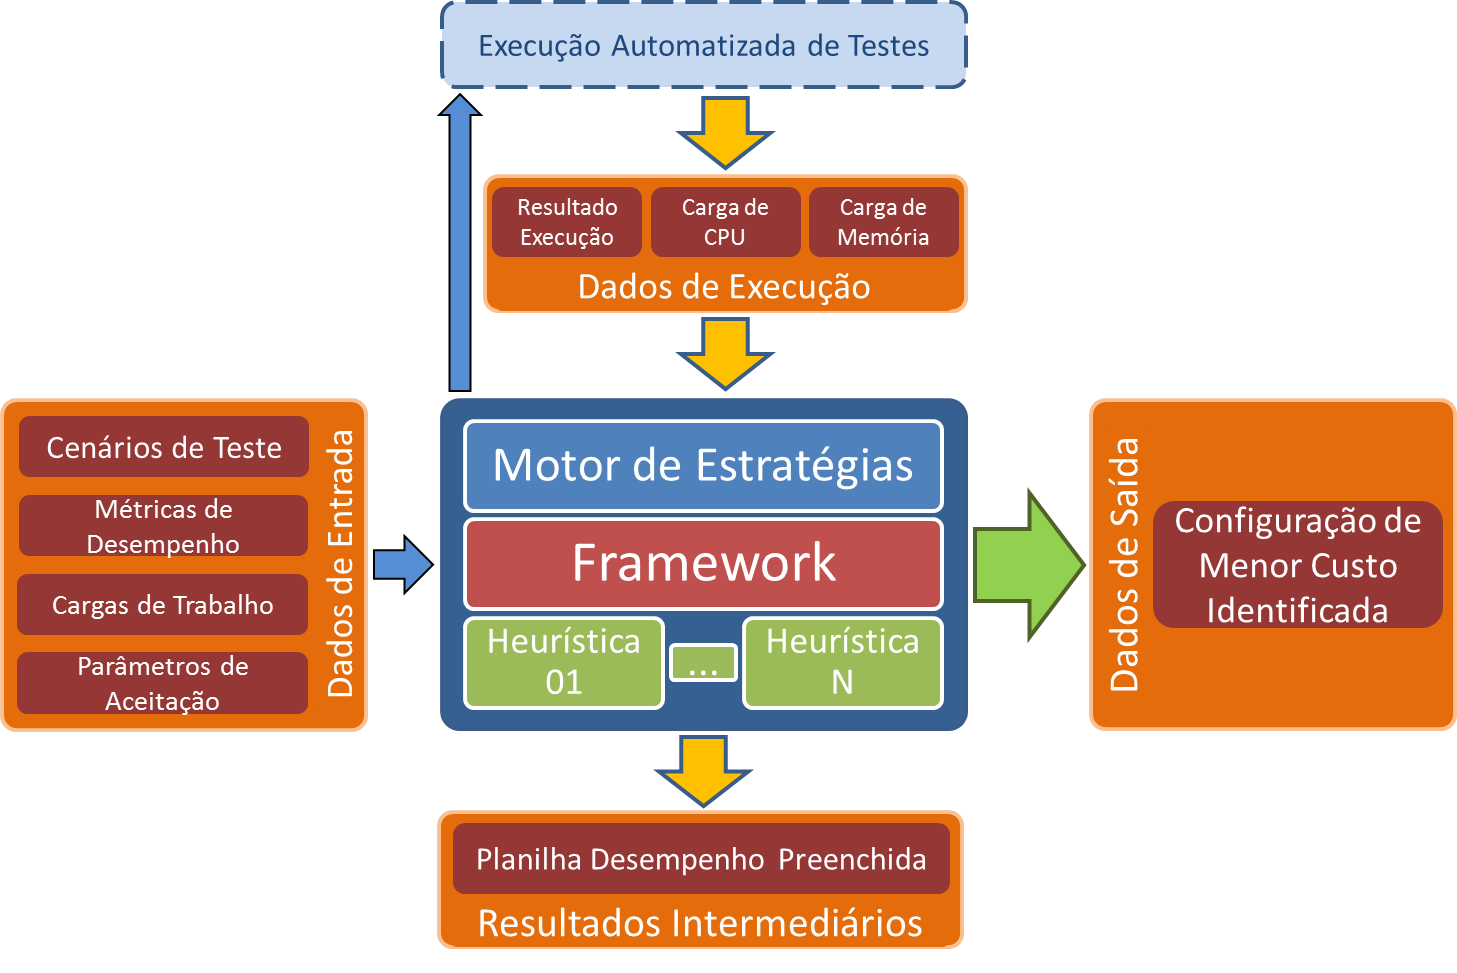
\includegraphics[scale=0.5]{img/arquiteturaAltoNivel}
  \end{center}
\end{figure}

As Heurísticas de Avaliação de Capacidade, conforme propostas neste trabalho, 
são implementações de estratégias que buscam encontrar, a partir do Resultado 
de uma Execução da Aplicação sob Teste sob uma Carga de Trabalho inicial em uma 
Configuração inicial, se existe uma Configuração mais barata que seja capaz de 
executar a mesma Carga de Trabalho.

O funcionamento de uma Heurística é totalmente baseado no caminhamento sobre o
Espaço de Implantação e sobre um a faixa de valores de Cargas de Trabalho. O 
tamanho de cada passo nesse caminho depende da lógica empregada pela Heurística 
e da avaliação do Resultado obtido. Cada passo dado pela Heuristica pode resultar 
em uma nova Execução dos testes ou em uma conclusão a respeito da capacidade da 
Configuração avaliada (e outras similares) de executar a Carga de Trabalho a um 
custo viável. Assim, a inteligência de uma Heurística está na forma como ela 
decide caminhar sobre o Espaço de Implantação e na faixa de Cargas de
Trabalho apresentados.

Apresentamos a seguir o modelo de como uma Heurística deve funcionar, a 
especificação do arcabouço de implementação construído nesse trabalho, começando
por descrever as operações que uma Heurística deve executar. 

\section{Operações Iniciais}
Para que uma Heurística de Avaliação de Capacidade seja compatível no âmbito deste trabalho, 
deve apresentar um conjunto mínimo de operações esperadas para que a lógica da
avaliação se complete e o resultado final obtido possa ser considerado válido e
comparável com os resultados obtidos por outras Heurísticas.

Além disso, as operações constituem a interface pela qual o controlador das 
sessões de avaliação pode configurar as Heurísticas e informar-lhe os dados 
necessários ao controle da sua execução.
 
Apresentamos esse conjunto mínimo de operações nas subseções a seguir, que 
representam o arcabouço necessário para a construção de uma Heurística de 
Avaliação de Capacidade.

\subsection{Selecionar Carga de Trabalho Inicial}
Este trabalho tem como premissa a necessidade de se identificar quais as 
Configurações mais baratas em um Provedor capazes de executar diversos níveis de
Cargas de Trabalho, tendo como objetivo a otimização de custos para a execução de
uma Aplicação so Teste.

Assim, pressupomos que exista uma faixa de valores para os níveis de Cargas de 
Trabalho a que a Aplicação é costumeiramente submetida e que seja de conhecimento
prévio dos responsáveis pela Aplicação. 

De posse dessa faixa de valores de Cargas de Trabalho, uma Heurística deve ser 
capaz de escolher, de acordo com sua estratégia de trabalho, um valor inicial de
Carga de Trabalho a ser imposta sobre a Aplicação. A Carga de Trabalho escolhida
deve ser retornada para o controlador da sessão, de forma que este possa coordenar
a Execução dos testes.
 
\subsection{Selecionar Configuração Inicial}
Analogamente, a fim de que as atividades da sessão de avaliação possam ter início,
é necessário que a Heurística de Avaliação de Capacidade usada selecione uma
Configuração inicial.

A escolha da Configuração inicial é feita a partir das Configurações disponíveis
no Espaço de Implantação previamente configurado pelo responsável pela avaliação.
A Heurística deverá avaliar o conjunto de configurações disponíveis quanto ao seu
preço, número de instâncias em cada, etc, de forma a escolher uma Configuração 
que considere mais adequada à sua estratégia para o início da sessão de avaliação.

\section{Operações de Controle}
Tendo em mãos uma Carga de Trabalho e uma Configuração iniciais, o controlador
da sessão de avaliação de capacidade pode ordenar uma Execução de testes, onde
serão coletados dados de desempenho relevantes para a Aplicação sob Teste.

Após a primeira Execução, um Resultado contendo os dados de desempenho colhidos 
é avaliado pelo controlador e, conforme sua decisão, novas Execuções podem se 
fazer necessárias. Neste caso, a Heurística deve ser novamente invocada, desta 
vez a selecionar uma nova Carga de Trabalho ou uma nova Configuração a partir do
Espaço de Implantação. Essa interação deve se repetir até que o controlador 
conclua os testes e dê por encerrada a sessão de avaliação.

Abaixo descrevemos as operações que a Heurística deve prover para que permita ao
controlador a correta operação dos testes e da sessão.

\subsection{Selecionar Nova Configuração}
Depois da cada execução de testes, o controlador estará de posse de um Resultado,
contendo os dados de desempenho da Aplicação executada sob a Carga de Trabalho e
a Configuração selecionadaa. A depender dos dados desse Resultado, o controlador
pode decidir executar novos testes em outra Configuração.

Para isso, a Heurística deve ser usada para selecionar a próxima Configuração a 
ser testada com a Aplicação. Com base no Resultado obtido pela Execução anterior,
a Heurística usará sua lógica de navegação para determinar a distância a ser 
caminhada no Espaço de Implantação em busca da nova Configuração.

A ordem de caminhamento é dada conforme a necessidade identificada pelo 
controlador, que vai definir se precisa de uma Configuração mais ou menos potente.
Porém, a Heurística é quem define, através de sua estratégia, qual será a próxima
Configuração usada.

Assim, a Heurística deve prover ao controlador duas operações para escolha da 
próxima Configuração: uma para Elevar o Nível de Configuração, ou seja, escolher
uma Configuração de capacidade superior, e outra para Reduzir o Nível de 
Configuração, isto é, escolher uma Configuração de capacidade inferior. Em ambos
os casos, a Heurística deverá usar como dado de entrada o Resultado da última 
Execução.

As Heurísticas são livres para usar os dados do Resultado como melhor lhe 
aprouverem, desde que a saída seja uma Configuração que ainda não tenha sido 
usada nos testes anteriores. 

\subsection{Selecionar Nova Carga de Trabalho}
De maneira similar à escolha de uma nova Configuração, o controlador pode usar
a Heurística para selecionar uma nova Carga de Trabalho, de acordo com o 
resultado com a última Execução.

As Heurísticas devem, então, prover operações que permitam a navegação pela
faixa de valores de Cargas de Trabalho estudada para a Aplicação sob Teste. 
Portanto, uma Heurística compatível deve fornecer duas operações de controle do
nível de Carga de Trabalho: uma operação para que seja reduzido e outra operação 
para que seja elevado o nível de Carga de Trabalho.

Aqui também as Heurísticas são livres para criarem suas próprias lógicas de 
avaliação dos dados do Resultado e, a partir daí, definirem qual o tamanho do
passo no caminhamento sobre a faixa de Cargas de Trabalho.
 
% ----------------------------------------------------------

% ----------------------------------------------------------

% ----------------------------------------------------------
% Solução
% ----------------------------------------------------------
\chapter[Esquema de Solução]{Esquema de Solução}
% ----------------------------------------------------------

***** DESCONSIDERAR POR ENQUANTO *****

O objetivo deste trabalho é estudar heurísticas de preenchimento da matriz P 
descrita no capítulo anterior sem necessariamente ter que executar de fato todos
os testes necessários. Esse preenchimento deverá ser feito, assim, por meio de 
um motor de predições que executará uma ou mais estratégias para preencher a 
matriz P com resultados calculados a partir dos dados de entrada.

Consideraremos como dados de entrada os resultados de uma ou mais execuções 
reais para um ou mais cenários de teste. A precisão dos resultados obtidos pelo 
motor de predição vai depender da qualidade da estratégia escolhida e da 
quantidade de dados de entrada. Quanto mais diversificadas quanto aos cenários a
que forem aplicadas e quanto maior o número de execuções reais usadas para 
alimentar inicialmente o motor de predições, mais preciso tenderá a ser o 
resultado da predição, porém mais caro se tornará o processo, uma vez que os 
testes executados no ambiente de nuvem incorrem em custo financeiro.

Apresentaremos um motor capaz de executar heurísticas de predição e um arcabouço
de implementação dessas heurísticas, de forma que nova inteligência de predição 
possa ser agregada ao trabalho futuramente. Apresentaremos também, como forma de
validar a proposta do arcabouço e do motor de execuções, duas heurísticas para 
geração da matriz P preenchida e sugestão da configuração de menor custo para 
executar a aplicação alvo em ambiente de nuvem de infraestrutura.


% ----------------------------------------------------------

% ----------------------------------------------------------
% ELEMENTOS PÓS-TEXTUAIS
% ----------------------------------------------------------
\postextual
% ----------------------------------------------------------

% ----------------------------------------------------------
% Referências bibliográficas
% ----------------------------------------------------------
\bibliography{dissertacao}

\end{document}
